\section{Clinical stratification} \label{clin}
% Note that this file describes only one implementation of the clinical stratification possible in the sm_sir code
\subsection{Stratification structure}
The ``clinical" stratification acts by replicating 
each of the two (age-stratified) sequential compartments representing infectious COVID-19 
into three categories (Figure \ref{fig:seeiir}).
These three clinical categories are:
\begin{enumerate}
    \item Asymptomatic persons
    \item Symptomatic persons who are never notified as cases
    \item Symptomatic persons who are successfully detected and notified
\end{enumerate}
For each age category, a proportion of new active infections are assumed to remain asymptomatic 
throughout their infectious period (first stratum, specified in Table \ref{tab:age_params}).
This proportion remains fixed over time throughout a model run.
We assumed that asymptomatic persons are never detected 
and so do not contribute to notifications.
The remaining proportion constitutes the second and third categories, 
comprising all persons who develop symptomatic COVID-19 during their infectious period.
The proportion of these symptomatic persons who progress to the third category 
can be allowed to vary with time,
but was fixed to remain constant for this application following discussions with local staff.
This approach differs from that presented in our previous COVID-19 modelling publications,
in that the earlier publications allowed for time-varying detection rates and
included additional stratification 
to distinguish those with detected COVID-19 according to disease severity.
By contrast, in this analysis, mortality and health service burden were calculated
by applying convolutions, as described below.
\begin{figure}[ht]
    \begin{center}
    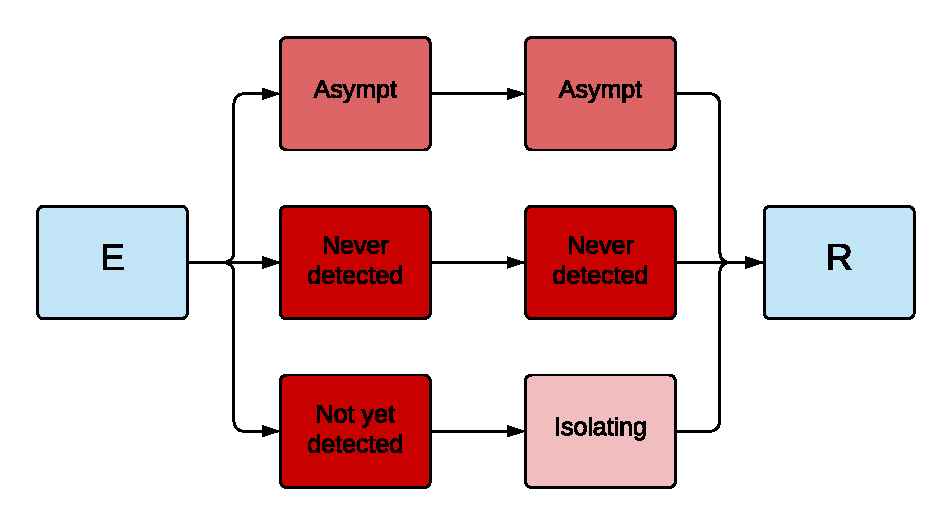
\includegraphics[width=0.7\textwidth]{../../tex_descriptions/models/sm_sir/stratifications/clinical_strat.pdf}
    \end{center}
    \caption{Illustration of the clinical stratification. \small Depth of red shading of compartment qualitatively indicates infectiousness.}
    \label{fig:seeiir}
\end{figure}
\subsection{Modification to infectiousness}
Both the early and late stages of the asymptomatic stratum 
of the infectious COVID-19 compartment are assumed to have 
partially reduced infectiousness,
according to the asymptomatic infectiousness parameter.
The late stage of the detected (third) stratum has reduced infectiousness 
to represent case isolation,
with these persons having their infectiousness reduced 
according to the isolation infectiousness parameter.
